%%%%%%%%%%%%%%%%%%%%%%%%%%%%%%%%%%%%%%%%%%%%%%%%%%%%%%%%%%%%%%%%%%%%%%%%%%%%%%%%
%2345678901234567890123456789012345678901234567890123456789012345678901234567890
%        1         2         3         4         5         6         7         8

\documentclass[letterpaper, 10 pt, conference]{ieeeconf}  % Comment this line out if you need a4paper

%\documentclass[a4paper, 10pt, conference]{ieeeconf}      % Use this line for a4 paper

\IEEEoverridecommandlockouts                              % This command is only needed if 
                                                          % you want to use the \thanks command

\overrideIEEEmargins                                      % Needed to meet printer requirements.

%In case you encounter the following error:
%Error 1010 The PDF file may be corrupt (unable to open PDF file) OR
%Error 1000 An error occurred while parsing a contents stream. Unable to analyze the PDF file.
%This is a known problem with pdfLaTeX conversion filter. The file cannot be opened with acrobat reader
%Please use one of the alternatives below to circumvent this error by uncommenting one or the other
%\pdfobjcompresslevel=0
%\pdfminorversion=4

% See the \addtolength command later in the file to balance the column lengths
% on the last page of the document

% The following packages can be found on http:\\www.ctan.org
\usepackage{graphics} % for pdf, bitmapped graphics files
\usepackage{xcolor} % for coloring
\usepackage{epsfig} % for postscript graphics files
\usepackage{booktabs} % for tables
\usepackage{multirow} % for tables
\usepackage{mathptmx} % for math equations
\usepackage{amsmath} % for math equations
\usepackage{amssymb}
\usepackage{float}
\usepackage{url}
\usepackage{hyperref}

\title{\LARGE \bf
Evaluating the Effectiveness of Haptic Force Feedback during Data Collection for Force-Aware Visuomotor Policy Learning
}


\author{Student Name$^{1,2}$, Student Name$^{1,2}$, Student Name$^{1,2}$, Student Name$^{1,2}$, Mentor Name$^{1}$, Mentor Name$^{1}$ \\
$^{1}$National Research Council Canada \quad
$^{2}$University of Waterloo
}


\begin{document}



\maketitle
\thispagestyle{empty}
\pagestyle{empty}

%%%%%%%%%%%%%%%%%%%%%%%%%%%%%%%%%%%%%%%%%%%%%%%%%%%%%%%%%%%%%%%%%%%%%%%%%%%%%%%%
\begin{abstract}\textit{
Precise physical interaction is a significant challenge for visual imitation
learning methods such as Diffusion Policy. To handle contact-rich tasks, the
community has introduced advanced methods relying on complex neural architectures
and reactive control flows. However, these methods overlook a critical bottleneck
during data collection: standard teleoperation setups lack force feedback,
completely depriving human operators of the tactile sensation that we rely on
for precise manipulation. In this work, we propose a haptic-fused imitation
learning framework. By utilizing a 6-DoF wrist-mounted force-torque sensor and
a 3-DoF Haply haptic controller, we allow human operators to physically feel
contact events through their fingertips during demonstration collection. We then
conduct a comparative study across three conditions on contact-rich tasks,
isolating the impact of haptic feedback on demonstration quality and resulting
policy performance. Our preliminary evaluation reveals that task selection is a
critical and underexplored variable: tasks where contact force is recoverable
from visual cues alone may not expose the advantage of haptic-fused data
collection, motivating a more principled benchmark for contact-rich policy
learning. Code, video, and dataset available at \url{TODO}.
}\end{abstract}

%%%%%%%%%%%%%%%%%%%%%%%%%%%%%%%%%%%%%%%%%%%%%%%%%%%%%%%%%%%%%%%%%%%%%%%%%%%%%%%%
\section{INTRODUCTION}
Contact-rich manipulation---tasks that require precise, continuous regulation 
of force exerted on objects---represents a fundamental challenge in robotics. 
This includes tight-tolerance plug-in-hole tasks such as connecting a USB cable, 
surface-following tasks such as cleaning a whiteboard, and deformable object 
interactions such as flattening clothes. Unlike pick-and-place, these tasks demand 
not only spatial precision but also real-time adaptation to contact dynamics that 
are difficult to model explicitly.

Visual imitation learning (IL) offers a promising route: robots learn directly 
from human demonstrations without task-specific programming. Methods such as 
Diffusion Policy~\cite{chi2024diffusionpolicy} and Action Chunking 
Transformer~\cite{zhao2023act} effectively capture the temporal structure of 
natural human behavior and have shown strong performance on a range of 
manipulation tasks. Reinforcement learning (RL) 
methods~\cite{luo2024serl,luo2024hilserl,rajeswaran2018dexterous} extend this 
further through online policy refinement seeded by demonstrations. However, 
these approaches ground the robot's perception entirely in vision---a modality 
that carries no information about physical contact forces, leaving them 
ill-equipped for contact-rich scenarios.

Yet one limitation persists across all of these approaches: force data recorded
at the robot's wrist during teleoperation is used to train the policy, but is
never fed back to the human operator during collection. The operator remains
entirely force-blind, relying solely on visual observation to judge contact
quality. Despite some efforts toward passive mechanical coupling through
leader-follower arms~\cite{zhao2023act} or instrumented gloves~\cite{liu2025forcemimic},
active haptic rendering---where the operator physically feels scaled contact forces
through a dedicated device---remains absent from the IL data collection pipeline.
This is consequential: in fine-grained contact-rich tasks, humans depend on
tactile sensation to modulate force, detect slip, and recover from failed contact.
Without it, demonstrations may carry errors in force regulation, setting a hard ceiling 
for force-aware policy learning frameworks.

In this work, we propose a haptic-fused imitation learning framework that closes
the sensory loop across the entire pipeline, from data collection through training
to inference. Using a 6-DoF wrist-mounted force-torque sensor paired with a 3-DoF
Haply Inverse3 haptic controller, we stream scaled contact forces from the robot's
end-effector directly to the operator's fingertips in real time. We evaluate three
experimental conditions: (1) a \textit{force-blind} baseline with no haptic
feedback and no force input to the policy; (2) a \textit{force-aware} policy
trained on force-blind demonstrations; and (3) our full \textit{haptic-fused}
pipeline with haptic-enabled demonstrations feeding a force-aware policy.
Preliminary results on two contact-rich tasks show no statistically significant
performance gap across conditions. 

Our contributions are as follows: we present
a complete, open-source haptic teleoperation infrastructure for end-to-end
haptic-fused demonstration collection; we provide an empirical datapoint
suggesting that on tasks where contact force is recoverable from visual cues,
haptic feedback yields no significant benefit. This motivates
more careful task selection in the future, and we introduce \textit{force-observability} as
a criterion for benchmarking contact-rich IL, identifying candidate tasks
(Section~\ref{sec:fut}) where closing the haptic loop is expected to produce
a measurable difference.

\begin{figure*}[t]
    \centering
    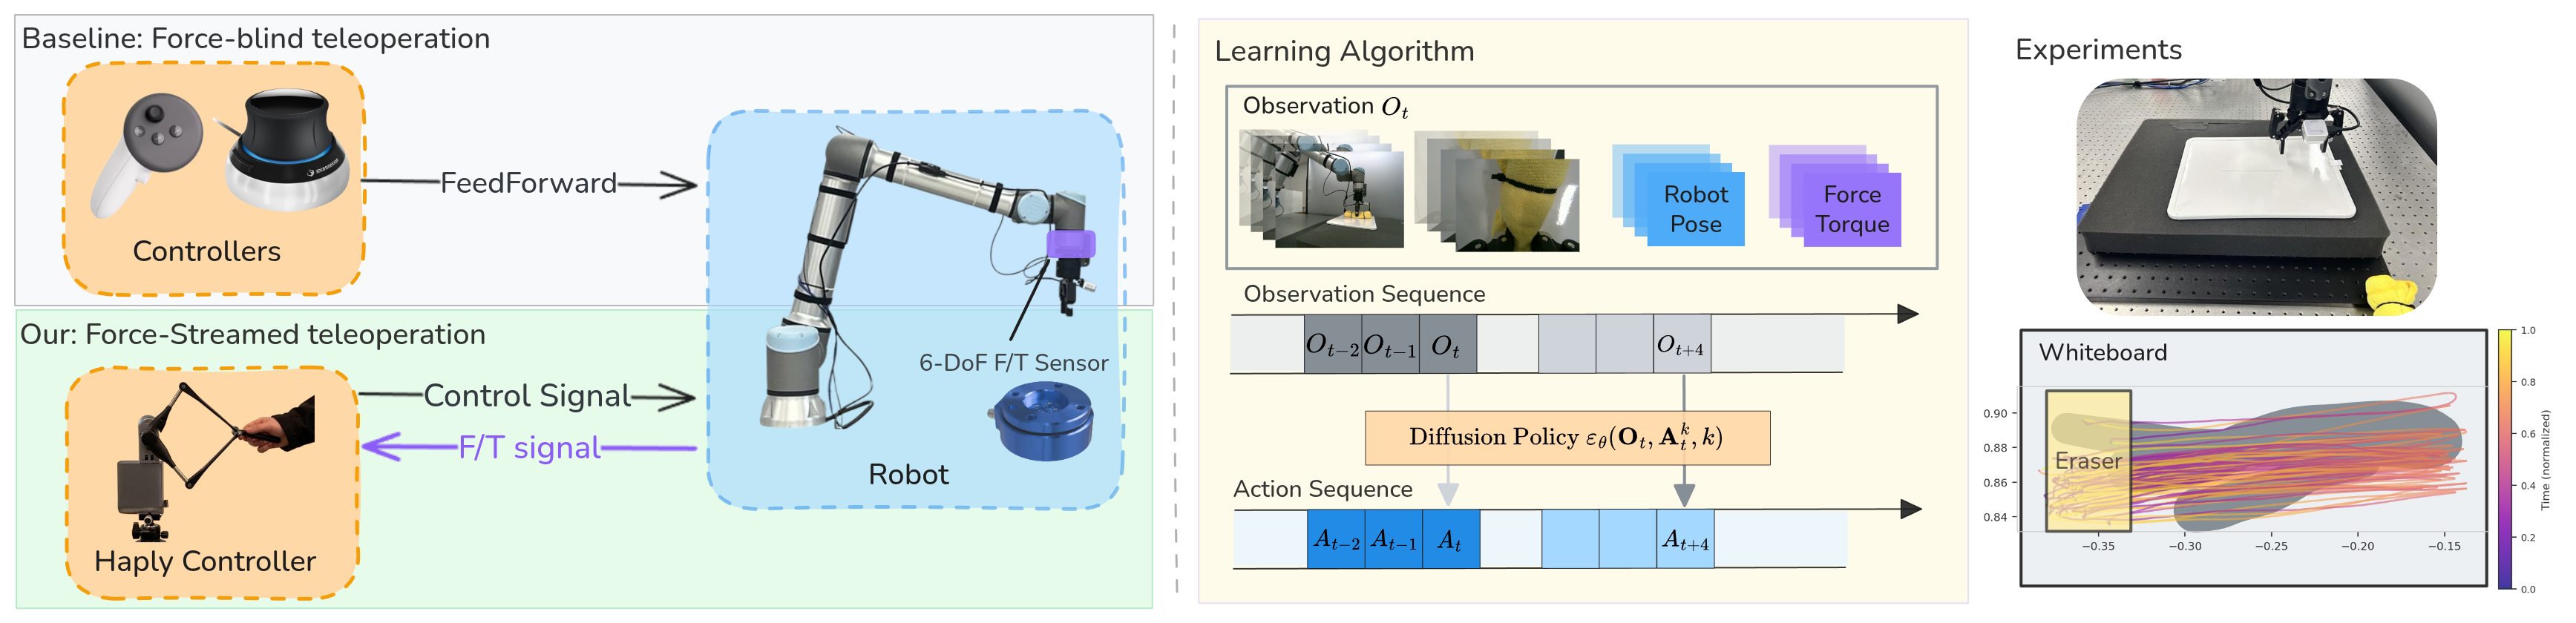
\includegraphics[width=\textwidth]{figures/Drawing.png}
    \caption{\textbf{Overview of the haptic-fused imitation learning framework.}}
    \label{fig:overview}
\end{figure*}

%%%%%%%%%%%%%%%%%%%%%%%%%%%%%%%%%%%%%%%%%%%%%%%%%%%%%%%%%%%%%%%%%%%%%%%%%%%%%%%%
\section{METHODOLOGY}

\subsection{Hardware}
% some of this very similar to previous paper - do we need to change wording?


% hardware:
A Universal Robots UR10e is controlled through the Real-Time Data Exchange (RTDE) interface for low-latency state feedback and command execution. Teleoperation is performed using a Haply Inverse3 with a VerseGrip attachment to capture 6-DoF operator inputs. A Robotiq parallel gripper enables object ineraction, while Intel RealSense cameras provide visual observations, one wrist mounted, one fixed for external view. Contact dynamics are measured using a 6-DoF MAE SensuReal force-torque sensor at the robot interface. 

\subsection{Teleoperation Pipeline}
% during data collection control loop (general; not involving haptic feedback):
At each control cycle, the system synchronously acquires robot states, operator inputs, and visual observations to ensure temporally consistent multimodal data. Incremental translational and rotational deltas from the haptic interface are integrated within the control loop to generate a target 6-DoF end-effector pose. Concurrently, the system records the corresponding proprioceptive states and force-torque measurements. Visual data are captured in parallel and temporally aligned via timestamp-based resampling onto a unified control-time grip. Each demonstration is stored as a time-indexed Zarr replay buffer entry. 

% force integration + haptic feedback implementation:

The haptic feedback pipeline (Fig. 1.) establishes a bidirectional coupling between the robot and the operator by mapping measured interaction forces to feedback at the input device. Force–torque measurements from the robot end-effector are processed within the control loop to produce a Cartesian force signal representing contact with the environment. This signal conveys interaction dynamics to the operator in real time.

To ensure stability and consistency, the force signal is conditioned prior to rendering. Low-pass filtering attenuates sensor noise, while rate limiting prevents abrupt transients. A virtual contact model based on a unilateral spring–damper formulation regulates interaction along the contact axis, with force thresholds governing engagement and disengagement. A blending mechanism ensures smooth transitions between free-space motion and contact.

The resulting force is scaled and transmitted to the haptic device, where it is rendered to the operator. This closes the loop: operator motion defines the robot’s desired state, and measured forces are returned as feedback to guide subsequent input.

%In the bilateral teleoperation control, the raw force-torque measurements are transformed to TCP-aligned coordindate frames and then aligned to the Haply coordinate frame. Within the force feedback loop, the force components of the Haply-aligned force is processed through low-pass filtering, rate limiting, and optional virtual wall rendering along the z-axis. The free-space and contact forces are then blended to produce a smooth feedback signal which is transmitted to the haptic device, enabling real-time force perception during teleoperation.

% \begin{figure*}[t]
%     \centering
%     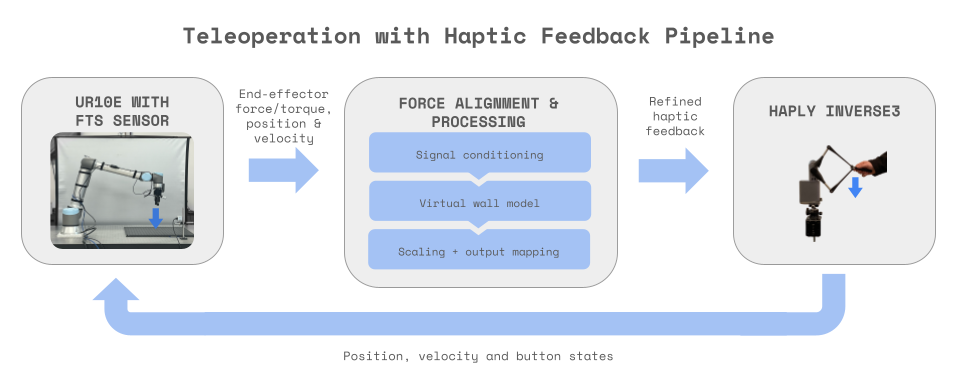
\includegraphics[width=\textwidth]{figures/TeleoperationPipeline.png}
%     \caption{Teleoperation pipeline}
%     \label{fig:teleop_pipeline}
% \end{figure*}

\subsection{Task Design}


In the data acquisition pipeline, we compare unilateral (w/o haptic feedback) and bilateral (w/ haptic feedback) teleoperation modes. Dataset quality is evaluated based on how effectively demonstrations capture the operator's understanding of environment dynamics and object properties. This is quantified through the analysis of the recorded force signals under each condition, and further assessed via end-effector trajectories, which directly reflect the operator's ability to execute stable, safe, consistent interactions and informed control decisions.

Applied force throughout episode: Comparing the exerted normal force in the z-axis (Fz) throughout the episode and the maximum exerted force. With the haptic feedback, the operator has more feedback on the teleoperation environment 

We consider various manipulation tasks with distinct contact interaction characteristics. The bottle-cap press task emphasizes the requirement for sensitivity to object mechanical properties. The operator is required to apply sufficient force to fully depress it avoiding damage. The second task, whiteboard wiping, involves sustained contact and emphasizes consistent force regulation throughout the interaction. The operator is required to maintain appropriate normal force while traversing the surface to effectively remove marker traces, thereby reflecting an understanding of surface properties and environmental constraints. 
We then compare the policy performance, with and without haptic feedback, to observe the downstream effects of uni- vs bi-lateral teleoperation modes.

We then compare the policy performance, with and without force-torque information as input in the diffusion policy training. 

\subsection{Policy Architecture}
The policy architecture is based on the original diffusion policy architecture pipeline [CITATION]. 
% dataset preprocessing + observation encoder
The absolute end-effector observation and action pose are converted into a pose-relative representation using the start pose. We train a conditioned diffusion policy that predicts an action trajectory from multi-view RGB and proprioceptive observations. 
The global conditioning vector is produced through the observation encoder that takes a specified number of observation steps (4 steps). For the image encoder, each RGB camera stream is passed through its own ResNet 18 backbone with the classification head removed. Then the preprocessed low dimensional signals are concatenated directly to the visual feature vector. This includes the conditional force-torque information recorded during data collection. 

% network policy
The global condiitioning vector is then passed into a CNN-based diffusion policy where the diffusion model is applied over action sequences implemented as a 1D convolutional U-Net over time. The Gaussian noise, which represents a whole action trajectory over a specified horizon length (16) is iteratively denoised with the conditional 1D U-Net. 

% inference pipeline

%%%%%%%%%%%%%%%%%%%%%%%%%%%%%%%%%%%%%%%%%%%%%%%%%%%%%%%%%%%%%%%%%%%%%%%%%%%%%%%%
\section{EXPERIMENTS AND RESULTS}
We perform experiments answering the following questions:
1) Does including haptic feedback during data collection improve dataset quality
2) Does including haptic feedback during data collection improve policy performance
3) Does including force-torque information as input in the diffusion policy improve policy performance
Environment. 
Tasks.
Evaluation Metrics.
a) Dataset quality
We 
b) Policy performance
\subsection{Dataset Quality Comparison}
\begin{figure}
    \centering
    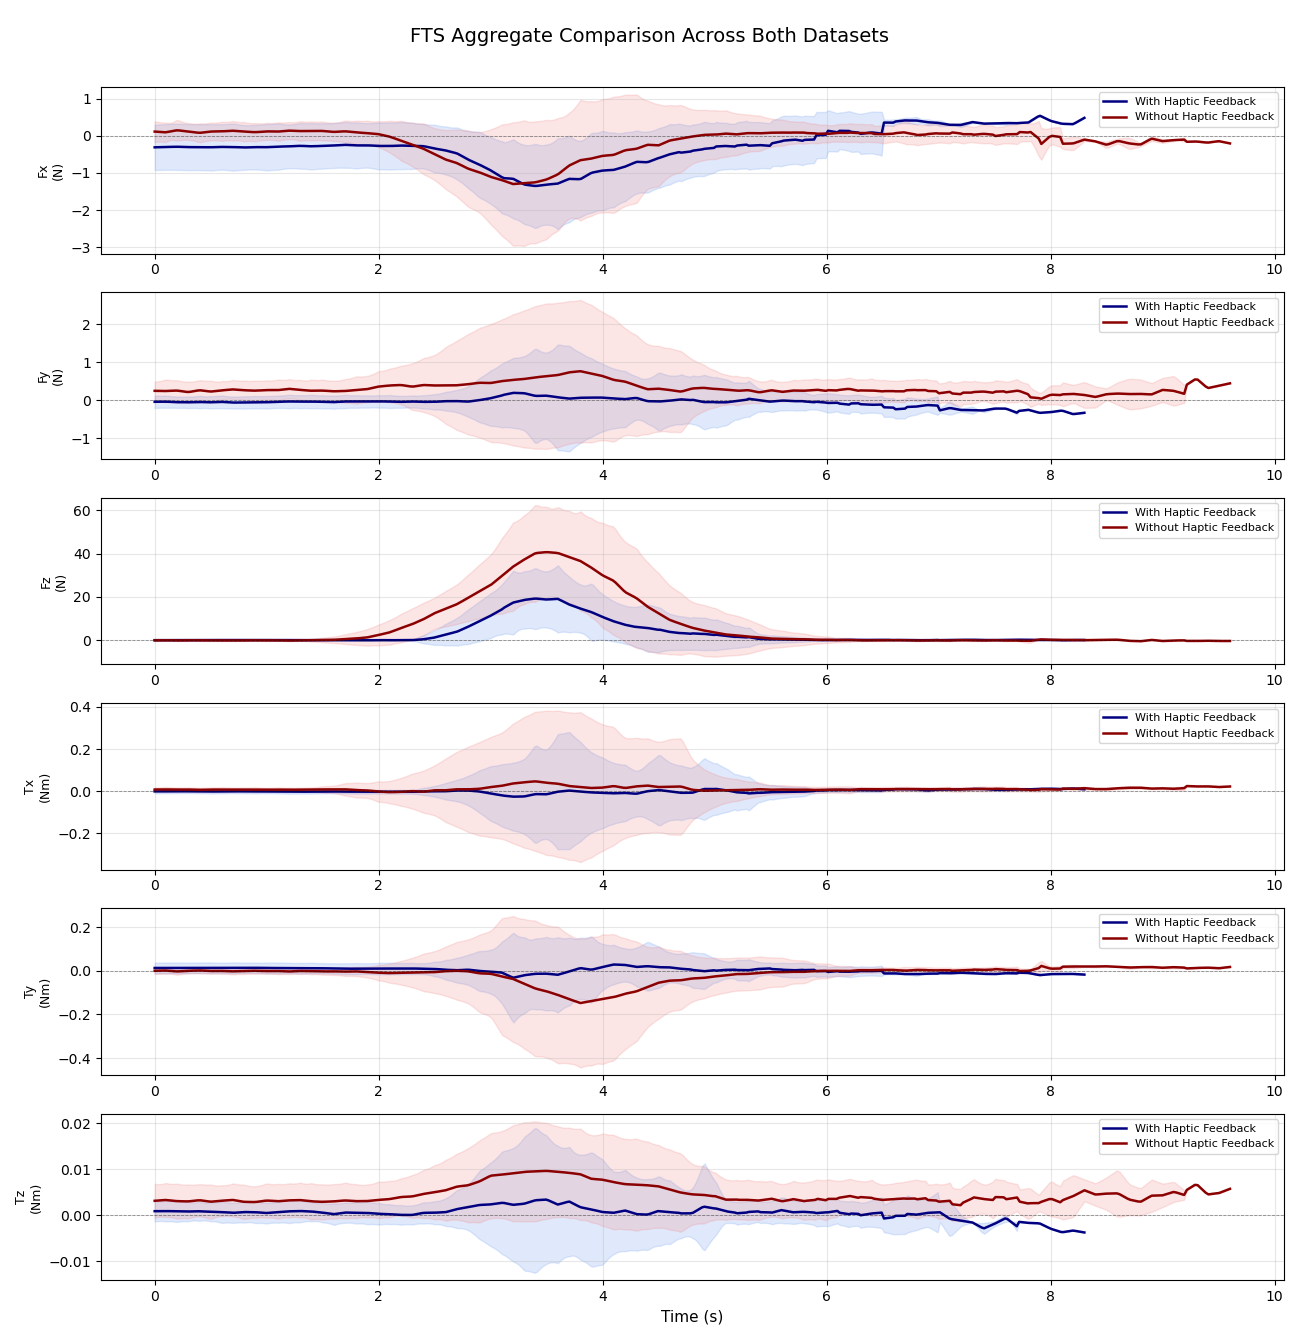
\includegraphics[width=0.5\linewidth]{figures/press_feedback_compare_force.png}
    \caption{Enter Caption}
    \label{fig:placeholder}
\end{figure}
Datasets collected with haptic feedback show lower normal contact force during the bottle-cap press than datasets collected without haptic feedback while maintaining consistency. This is shown using these metrics:

To characterize the normal force (Fz) applied during the contact phase, we computed the mean Fz across all episodes, with the corresponding standard deviation (+- 1 SD) bands shown to represent inter-episode variability. Figure X reveals that the mean Fz with haptic feedback is substantially lower than without haptic feedback throughout the primary contact region, with peak forces reduced from approximately x N to y N. The standard deviation bands remain comparably in width between both conditions suggesting that the lower normal forces were applied in a controlled and repeatable manner rather than a result from uncontrolled modulation. 
% probably discussion:
These results indicate that haptic feedback enabled users to regulate normal force application more effectively, maintaining consistent task execution while reducing applied force magnitude.

To further visualize the maximum external force in each episode, a boxplot is used. It is evident that the haptic-feedback dataset has more consistent peak forces and a lower median for the peak force compared to the dataset without haptic feedback. 

Based on the force a human exerts on the bottle cap for daily usage, a baseline range for a reasonable amount of force was determined to be approximately 15N to 30N. It is evident in the data collection, with the haptic device, this was the average normal force exerted was within this range. 

\begin{figure}[H]
    \centering
    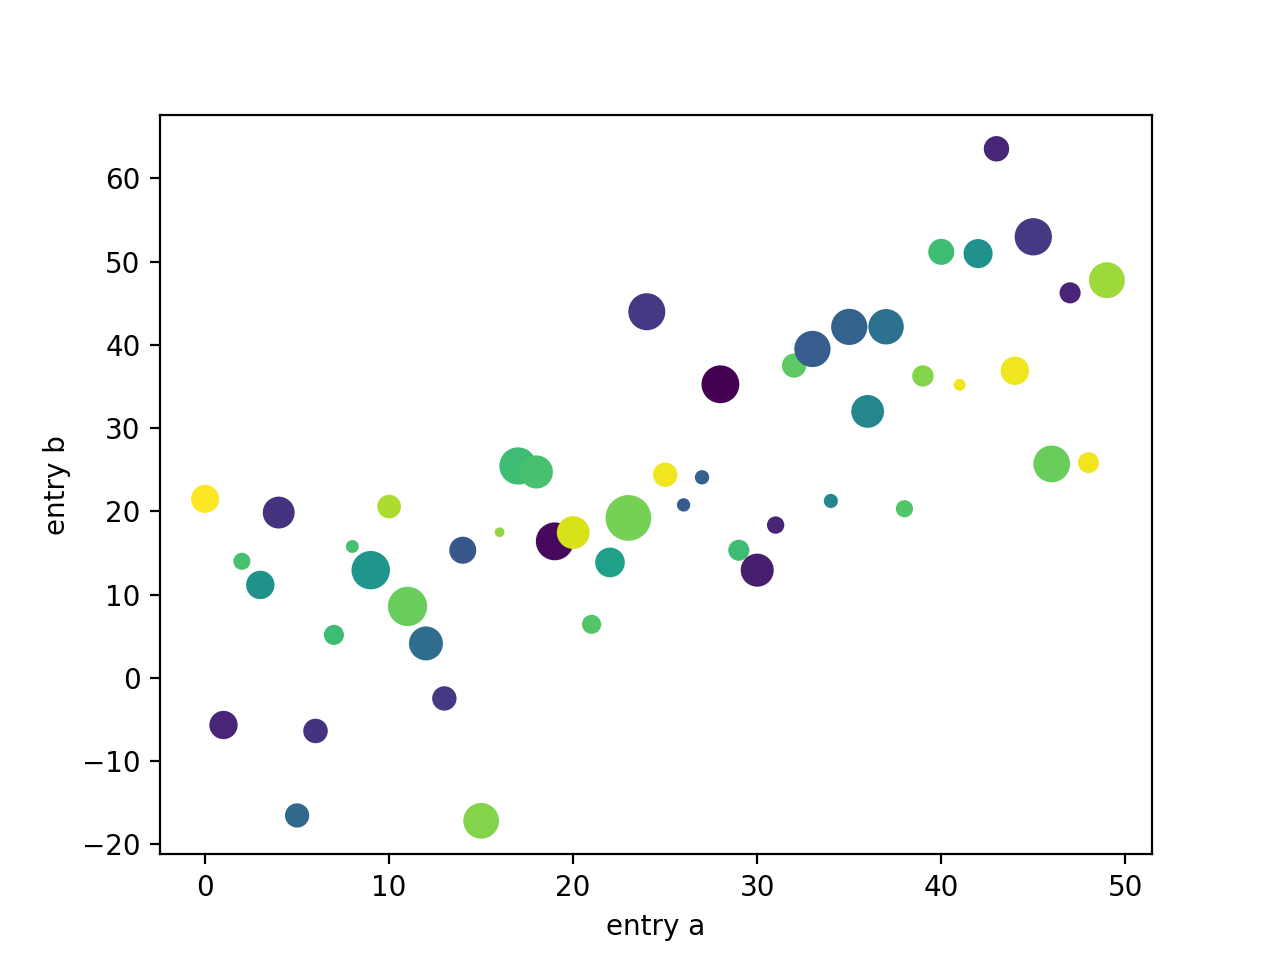
\includegraphics[width=150pt]{figures/Example.png}
    \caption{Example Figure}
    \label{figurelabel}
\end{figure}

%%%%%%%%%%%%%%%%%%%%%%%%%%%%%%%%%%%%%%%%%%%%%%%%%%%%%%%%%%%%%%%%%%%%%%%%%%%%%%%%
\subsection{Performance Analysis}

\begin{table}[H] 
    \centering
    \caption{Example Table for Quantitative Performance Evaluation}
    \label{tab:results}
    % Shrinks the table to fit perfectly inside the column
    \resizebox{\columnwidth}{!}{% 
    \begin{tabular}{@{} l c c c c @{}} 
        \toprule
        \multirow{2}{*}{\textbf{Condition}} & \multicolumn{2}{c}{\textbf{Balloon}} & \multicolumn{2}{c}{\textbf{Assembly}} \\
        \cmidrule(lr){2-3} \cmidrule(lr){4-5}
         & Succ. ($\uparrow$) & Force ($\downarrow$) & Succ. ($\uparrow$) & Force ($\downarrow$) \\
        \midrule
        Baseline & xx\% & xx N & xx\% & xx N \\
        \textbf{Ours} & \textbf{xx\%} & \textbf{xx N} & \textbf{xx\%} & \textbf{xx N} \\
        \bottomrule
    \end{tabular}%
    }
\end{table}

\section{DISCUSSION \& FUTURE WORK}

Discussion
- Haptic feedback helped moderate the amount of force; with a task that didn't require lots of force, the user was more easily able to tell when to stop, and with a task that required extra force, the user was able to consistently apply that amount of force.

and improved the consistency of force applied during tasks, showing that force feedback during teleoperation improves data collection quality


Future work
- Improving the integration of force data in the diffusion policy
    - Different input into the policy, or flipping back and forth between control methods, or scaling the output of the policy with the inputed force feedback
- Testing across a wider range of tasks requiring force
- 
\label{sec:fut}

%%%%%%%%%%%%%%%%%%%%%%%%%%%%%%%%%%%%%%%%%%%%%%%%%%%%%%%%%%%%%%%%%%%%%%%%%%%%%%%%
\section{CONCLUSIONS}

This is to conclude our paper. 

\newpage



% %%%%%%%%%%%%%%%%%%%%%%%%%%%%%%%%%%%%%%%%%%%%%%%%%%%%%%%%%%%%%%%%%%%%%%%%%%%%%%%%

% References are important to the reader; therefore, each citation must be complete and correct. If at all possible, references should be commonly available publications.

\clearpage

\bibliographystyle{IEEEtran}
\bibliography{references}


\end{document}